\section{Results}
\label{sec:results}

\subsection{Fixed Cutoffs Alter Measured Effects}

Table~\ref{tab:fixed-l} shows that fixed Top-$L$ fusion can change both
retrieval scores and the ordering of query constructions. At $L=50$, Shared
expansion exceeds the sparse binary mask in macro nDCG@10 (.4641 vs.\ .4639),
whereas the ordering reverses under complete-list fusion (.4671 vs.\ .4675).
This shows that method comparison depends on the selected cutoff.

\begin{table*}[t]
\centering
\scriptsize
\setlength{\tabcolsep}{2.7pt}
\begin{tabular}{lrrrrrrrr}
\toprule
Method & $L=10$ & $L=20$ & $L=50$ & $L=100$ & $L=200$ & $L=500$ & $L=1000$ & Complete \\
\midrule
No expansion        & .4478 & .4489 & .4512 & .4553 & .4565 & .4569 & .4571 & \textbf{.4572} \\
Shared              & .4630 & .4633 & .4641 & .4645 & .4666 & .4670 & \textbf{.4671} & \textbf{.4671} \\
Dense only          & .4566 & .4568 & .4582 & .4608 & .4617 & \textbf{.4622} & .4621 & .4621 \\
Sparse only         & .4661 & .4676 & .4654 & .4686 & .4704 & .4713 & \textbf{.4715} & .4714 \\
MuGI-style (controlled) & .4612 & .4615 & .4608 & .4613 & .4630 & .4636 & .4637 & \textbf{.4638} \\
Sparse binary mask  & .4635 & .4637 & .4639 & .4649 & .4670 & .4672 & \textbf{.4675} & \textbf{.4675} \\
Reference-only sparse & .4534 & .4537 & .4529 & .4537 & .4555 & .4559 & .4564 & \textbf{.4565} \\
DESA                & .4738 & .4727 & .4709 & .4727 & .4740 & .4743 & \textbf{.4747} & \textbf{.4747} \\
\bottomrule
\end{tabular}
\caption{Equal-dataset macro nDCG@10 under fixed top-$L$ and complete-list
fusion on the seven evaluation datasets. Bold marks the maximum within each
row.}
\label{tab:fixed-l}
\end{table*}

The fused rankings at practical cutoffs also differ substantially from their
complete-list targets. Across the eight constructions, exact agreement with
the complete-list ordered Top-20 ranges from 0.04\% to 2.02\% at $L=20$ and
from 12.35\% to 16.54\% at $L=50$. Even at $L=1000$, fixed-cutoff fusion does
not always reproduce the complete-list result.

The effect is clearer at the individual-query level. For DESA versus Original,
$L=50$ assigns a different gain, tie, or loss label to 6.95\% of query and
generation-draw pairs under nDCG and 18.84\% under Recall. Strict gain-to-loss
or loss-to-gain reversals occur for 3.07\% and 3.06\%, respectively. At
$L=100$, label changes remain at 2.17\% for nDCG and 11.74\% for Recall.
Fixed-$L$ evaluation can therefore change the conclusion for individual
queries even when macro scores remain stable.

\subsection{Retrieval Effectiveness and Access Depth}

Under complete-list fusion, DESA obtains the highest macro nDCG@10 and
Recall@20 in the seven-dataset controlled comparison, reaching .4747 and
.4695. Relative to Original, these values correspond to gains of 3.82\% and
2.38\%. The equal-dataset averages of the within-dataset depth reductions are
36.90\% for Dense and 36.56\% for Sparse. The mean proportion of queries that
become shallower in both channels is 63.31\%. All four improvements remain
significant after Holm correction ($p_{\mathrm{Holm}}=.0004$).

\begin{table}[t]
\centering
\small
\setlength{\tabcolsep}{3.5pt}
\begin{tabular}{lrrrr}
\toprule
Method & nDCG@10 & Recall@20 & $L_D$ & $L_S$ \\
\midrule
No expansion & .4572 & .4586 & 1752.4 & 1455.1 \\
Shared       & .4671 & .4666 & \textbf{607.4} & \textbf{606.7} \\
Dense only   & .4621 & .4637 & 1386.5 & 1219.9 \\
Sparse only  & .4714 & .4678 & 884.4 & 822.0 \\
DESA         & \textbf{.4747} & \textbf{.4695} & 728.9 & 673.2 \\
\bottomrule
\end{tabular}
\caption{Equal-dataset macro results for the seven-dataset controlled
comparison. Higher is better for retrieval metrics; lower is better for replay
stopping depths. Raw depths are averaged across datasets; percentage reductions
in the text are computed within each dataset before macro-averaging.}
\label{tab:main-results}
\end{table}

Compared with Shared expansion, DESA improves macro nDCG by 1.61\% and Recall
by 0.61\%. The absolute nDCG difference is $+.0075$ and remains significant
after correction ($p_{\mathrm{Holm}}=.0012$). The Recall difference is $+.0028$
($p_{\mathrm{Holm}}=.2736$), while the differences in Dense and Sparse depth
are also nonsignificant. DESA therefore provides a significant nDCG advantage
over Shared expansion.

NFCorpus illustrates the effect of Sparse anchoring. Shared expansion increases
the mean Sparse support from 561.5 to 3211.6 documents and raises Sparse
stopping depth by 105.82\% relative to Original. DESA preserves the original
support size and reduces Sparse depth by 23.15\%, while also reducing Dense
depth by 15.03\%. Anchoring allows generated terms to improve the ordering of
originally matched documents without expanding the lexical support.

\subsection{Contributions of the Channel Operators}

The $2\times2$ experiment shows that the two channel operators are
complementary. Dense residual expansion alone improves nDCG and Recall by
1.08\% and 1.11\%, with Dense and Sparse depth reductions of 8.16\% and 7.49\%.
Sparse anchoring alone produces larger quality gains of 3.11\% and 2.01\%,
together with depth reductions of 28.77\% and 27.74\%. Combining both operators
gives the full DESA gains of 3.82\% and 2.38\%, while reducing Dense and Sparse
depth by 36.90\% and 36.56\%.

Sparse anchoring contributes most of the quality gain, while Dense residual
expansion further reduces access depth. Their isolated controls produce only
small differences, whereas the complete channel-asymmetric construction
significantly outperforms Shared expansion in nDCG. DESA's advantage therefore
comes from combining the two channel-specific operations.

\begin{figure*}[t]
\centering
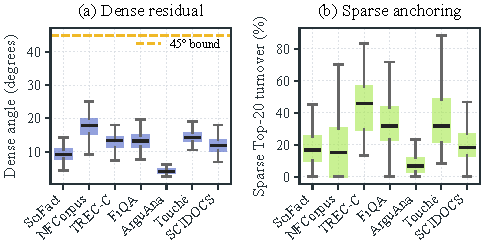
\includegraphics[width=\textwidth]{figures/fig_mechanism_distributions.pdf}
\caption{Realized behavior of the two channel operators over three generation
draws on seven datasets. Dense angles are measured from the original query;
Sparse turnover is one minus Top-20 overlap with the original sparse ranking.
Boxes show the interquartile range and median; whiskers extend to 1.5 times the
interquartile range, with outliers omitted.}
\label{fig:mechanism-distributions}
\end{figure*}

The observed rankings confirm the intended channel behavior
(Figure~\ref{fig:mechanism-distributions}). Across 11,327 query and
generation-draw pairs, the mean Dense angle is $11.98^\circ$, and the maximum
is $27.87^\circ$, below the analytic $45^\circ$ bound. Sparse anchoring changes
26.15\% of the original Sparse Top-20 on average. Relevant-document
reciprocal-rank gain correlates more strongly with Sparse-only nDCG gain than
overall Top-20 turnover does (.391 vs.\ .078). Sparse anchoring therefore
improves retrieval by promoting relevant documents within the original support,
while Dense residual expansion adds semantic evidence without excessive drift.

Additional binary-mask, reference-count, and operator-control results are
reported in Appendix~\ref{sec:appendix-analysis}.

\subsection{Comparison with Recent and Prior Methods}

Under matched generated evidence, QuDAR-simple RRF obtains .4761 nDCG and
.4714 Recall, compared with .4747 and .4695 for DESA. Neither paired difference
is significant after correction. QuDAR-simple fuses four Top-1000 rankings,
corresponding to 4,000 rank entries per query. DESA requires a mean of 1,402.1
entries to certify its fused result under the replay policy, a reduction of
64.95\%. DESA therefore matches the retrieval quality of the rank-based QuDAR
variant with substantially less fusion-side ranking access.

On the common four-dataset subset, DESA improves nDCG and Recall over HyDE by
16.58\% and 10.78\%, while reducing both stopping depths by about 91\%.
Relative to MuGI, the quality gains are 5.58\% and 2.92\%, and Dense and Sparse
depths decrease by 50.22\% and 51.77\%. DESA therefore outperforms both methods
in retrieval quality and ranking access under the shared evaluation protocol.

\begin{table}[t]
\centering
\small
\setlength{\tabcolsep}{3.5pt}
\begin{tabular}{lrrrr}
\toprule
Method & nDCG@10 & Recall@20 & $L_D$ & $L_S$ \\
\midrule
No expansion & .3325 & .5142 & 1278.2 & 1228.4 \\
HyDE         & .2956 & .4746 & 7918.3 & 7536.6 \\
MuGI         & .3264 & .5109 & 1409.0 & 1406.3 \\
Query2doc    & \textbf{.3461} & .5229 & 865.0 & 857.8 \\
DESA         & .3446 & \textbf{.5258} & \textbf{701.5} & \textbf{678.2} \\
\bottomrule
\end{tabular}
\caption{Equal-dataset macro comparison with prior query expansion methods
on the common four-dataset subset.}
\label{tab:fidelity}
\end{table}

Query2doc has 0.45\% higher nDCG, whereas DESA has 0.57\% higher Recall. DESA
also reduces Dense and Sparse stopping depths by 18.90\% and 20.93\%. The two
methods have similar retrieval quality, but DESA requires less ranking evidence
to determine the fused result.

\subsection{Robustness and Failure Boundary}

DESA retains its quality gains across the tested generator, Dense encoder, and
corpus sizes. Access depth decreases in most settings, with Contriever on
Touch\'e-2020 as the only observed failure case. Detailed generator, encoder,
and corpus-scale results are reported in Appendix~\ref{sec:additional-results}.
